\documentclass[conference]{IEEEtran}
\IEEEoverridecommandlockouts
\usepackage{cite}
\usepackage{amsmath,amssymb,amsfonts}
\usepackage{algorithmic}
\usepackage{flafter}
\usepackage{graphicx}
\usepackage{textcomp}
\usepackage{xcolor}
\usepackage{pdflscape}
\graphicspath{ {imagenes/} }

\begin{document}

\title{Actividad G.2\\Saltos
}

\author{\IEEEauthorblockN{Ricardo David López Arellano}
\IEEEauthorblockA{\textit{Departamento de Ingeniería en Computación} \\
\textit{CUCEI}\\
Universidad de Guadalajara\\
ricardo.lopez1361@alumnos.udg.mx}
}
\onecolumn

\maketitle

\begin{abstract}
Una estructura de datos tipo pila permite agregar nodos a la pila y eliminarlos de esta sólo desde su parte superior. Por esta razón, a una pila se le conoce como estructura de datos UEPS (último en entrar, primero en salir) o LIFO.
\end{abstract}

\begin{IEEEkeywords}
\begin{center}
Jump, jumpnz, jumpz, DS.
\end{center}
\end{IEEEkeywords}

\section{Originalidad}

Me comprometo a producir trabajo académico íntegro, lo que significa un trabajo que se adhiere a los estándares intelectuales y académicos de atribución exacta de las fuentes, uso y recolección de datos apropiados, y transparencia en el reconocimiento de las contribuciones de las ideas, descubrimientos, interpretaciones y conclusiones de otros.
Acepto que la trampa en los exámenes, el plagio o la fraudulenta representación de las ideas o lenguaje de otros como propio, la falsificación de datos o cualquier otra instancia de deshonestidad académica, violan los estándares de LA MATERIA, así como los estándares del mundo en general en el campo del conocimiento y las relaciones.

\section{Introducción}
\begin{center}
Las instrucciones de salto permiten cambiar la secuencia de ejecución de un programa.
\end{center}

\section{Objetivos de la actividad}
\begin{center}
• Cambiar la secuencia de ejecución de un programa mediante saltos.\\
• Implementar estructuras básicas utilizando saltos.
\end{center}

\section{Metodología}
Una pila (stack en inglés) es una lista ordenada o estructura de datos que permite almacenar y recuperar datos, siendo el modo de acceso a sus elementos de tipo LIFO (último en entrar, primero en salir). Esta estructura se aplica en multitud de supuestos en el área de la informática debido a su simplicidad y capacidad de dar respuesta a numerosos procesos.\\

Para el manejo de los datos cuenta con dos operaciones básicas: apilar (push), que coloca un objeto en la pila, y su operación inversa, retirar (o desapilar, pop), que retira el último elemento apilado.\\

En cada momento solamente se tiene acceso a la parte superior de la pila, es decir, al último objeto apilado. La operación retirar permite la obtención de este elemento, que es retirado de la pila permitiendo el acceso al anterior (apilado con anterioridad), que pasa a ser el último, el nuevo TOS.

\section{Contenido}
\subsection{Secuencia de ejecución:}
\begin{itemize}
\item Jump: palabra que salta a una dirección de memoria especificada por la etiqueta.
\item jumpnz: palabra que salta a una dirección de memoria especificada por la etiqueta cuando la celda superior de la pila de datos es un entero diferente a 0.
\item jumpz: palabra que salta a una dirección de memoria especificada por la etiqueta cuando la celda superior en la pila de datos es un entero igual a 0.
\end{itemize}

\section{Resultados (códigos)}
\begin{enumerate}
\item  EJERCICIO 1:\\
	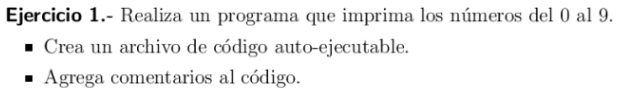
\includegraphics{e1} \\
	\begin{center}
	\textbf{Respuesta: } 0 . \\ 0 \\ etiqueta: //aqui metemos el codigo como un tipo "swtich" \\ 1 + \\ dup . //con dup duplicamos la celda superior de la pila \\ dup \\ 9 = \\ jumpz etiqueta
	\end{center}
	
\item  EJERCICIO 2:\\
	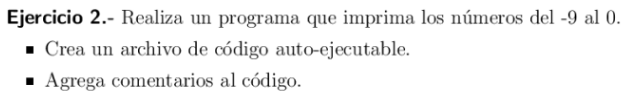
\includegraphics{e2} \\
	\begin{center}
	\textbf{Respuesta: } 9 -1 S* \\ S. \\ 9 \\ etiqueta: //aqui metemos el codigo como un tipo "swtich" \\ 1 - \\ dup -1 S* S. //Con la S imprimimos numeros negativos \\ dup //con dup duplicamos la celda superior de la pila \\ jumpz etiqueta //aqui mandamos llamar la etiqueta
	\end{center}
	
\item  EJERCICIO 3:\\
	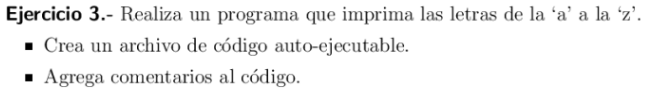
\includegraphics{e3} \\
	\begin{center}
	\textbf{Respuesta: } 97 emit //con emit imprimimos el numero en la celda top \\ 97 \\ etiqueta: \\ ++ \\ dup emit \\ dup \\ 122 = \\ jumpz etiqueta \newpage

	\end{center}
	
\item  EJERCICIO 4:\\
	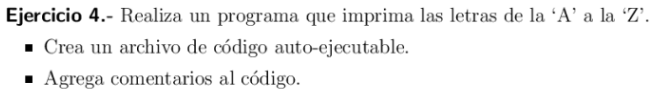
\includegraphics{e4} \\
	\begin{center}
	\textbf{Respuesta: } 65 emit \\ 65 \\ etiqueta: \\ ++ \\ dup emit \\ dup \\ 90 = \\ jumpz etiqueta \\ 
	\end{center}

\item  EJERCICIO 5:\\
	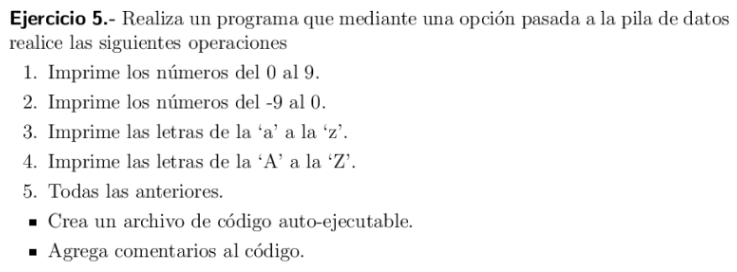
\includegraphics{e5}\\
	\begin{center}
	\textbf{Respuesta: } 4 \\ dup 1 = jumpnz funcion1 \\ dup 2 = jumpnz funcion2 \\ dup 3 = jumpnz \\ funcion3 \\ dup 4 = jumpnz funcion4 \\ funcion1: \\ 0 . \\ 0 \\ etiqueta: \\ 1 + \\ dup . \\ dup \\ 9 = \\ jumpz etiqueta \\ jump \\ Final \\ funcion2: \\ 9 -1 S* \\ S. \\ 9 \\ etiqueta1: \\ 1 - \\ dup -1 S* S. \\ dup \\ 0 = \\ jumpz etiqueta1 \\ jump \\ Final \\ funcion3: \\ 97 emit \\ 97 \\ etiqueta2: \\ ++ \\ dup emit \\ dup \\ 122 = \\ jumpz etiqueta2 \\ jump \\ Final \\ funcion4: \\ 65 emit \\ 65 \\ etiqueta3: \\ ++ \\ dup emit \\ dup \\ 90 = \\ jumpz etiqueta3 \\
	\end{center}

\end{enumerate}
\newpage
\section{Resultados (diagramas de flujo)}
\begin{enumerate}
  	\item EJERCICIO 1:\\
  	\begin{center}
	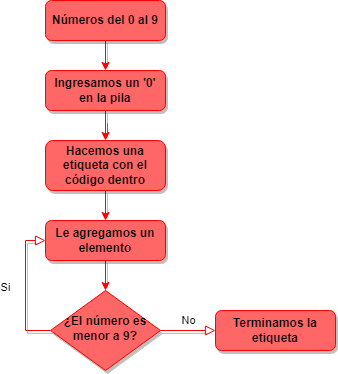
\includegraphics{diagrama1} 
	\end{center}
\newpage
	\item  EJERCICIO 2:\\
	\begin{center}
	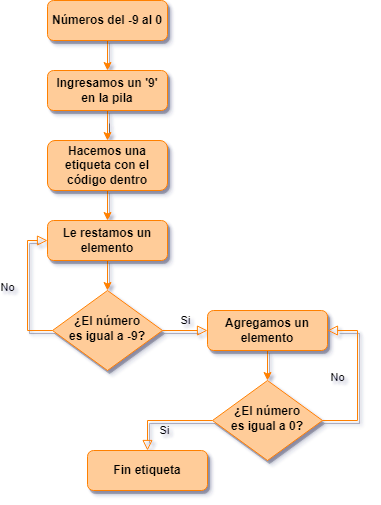
\includegraphics{diagrama2} \\
	\end{center}
\newpage	
	\item  EJERCICIO 3:\\
	\begin{center}
	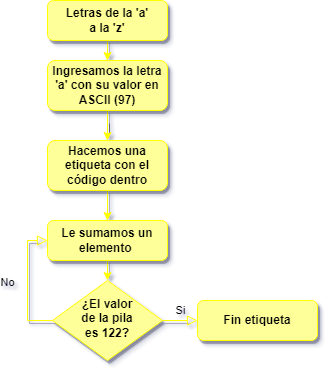
\includegraphics{diagrama3} \\
	\end{center}
\newpage	
	\item  EJERCICIO 4:\\
	\begin{center}
	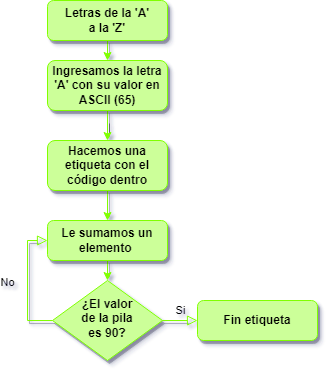
\includegraphics{diagrama4} \\
	\end{center}
	
	\item  EJERCICIO 5:\\
	\begin{center}
	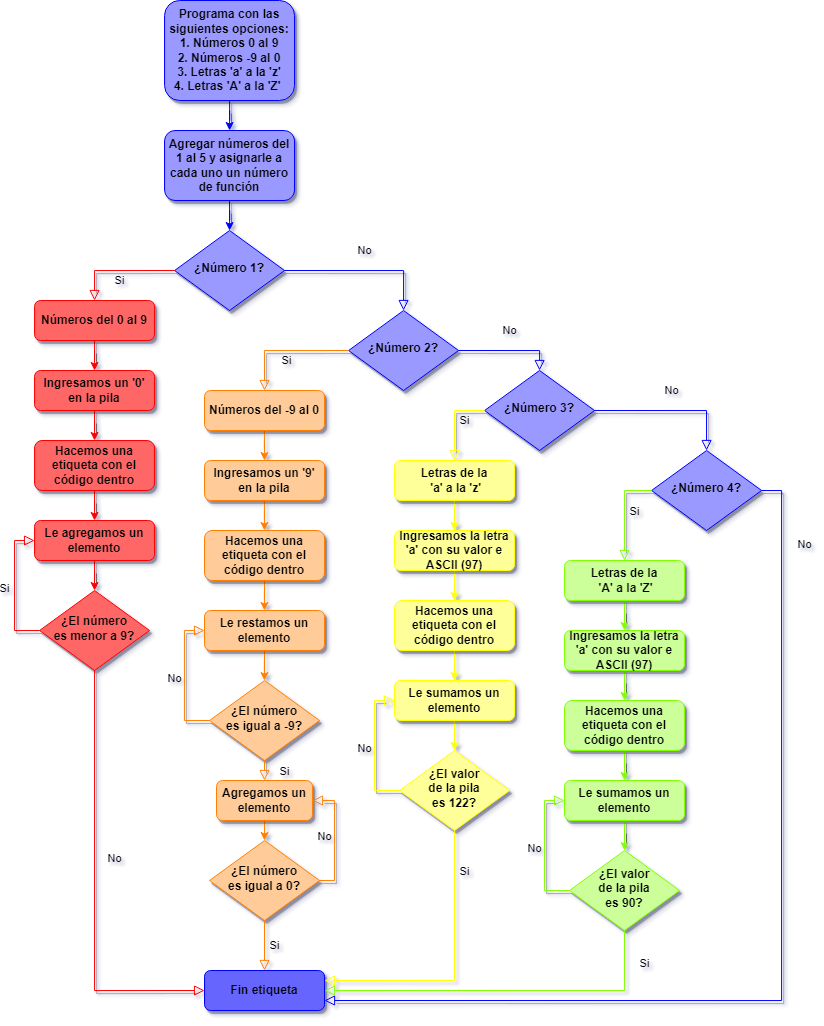
\includegraphics{diagrama5} \\
	\end{center}

\end{enumerate}
\newpage
\section{Conclusiones}  
En conclusión de esta tarea puedo decir que estos ejercicio fueron demasiados fáciles ya que no tenia mucha lógica realizarlos, pero como hemos ido avanzando se fueron complicando más. Pero es bueno aprender un lenguaje nuevo ya que yo ni si quiera había utilizado Linux ni mucho menos Latex, así que es una buena experiencia.

\section*{Agradecimientos}
Quiero hacer agradecimiento a mi profesor por explicarme cuando tenia dudas sobre cómo hacer los ejercicios, a mis compañeros porque varias veces me brindaron ayuda cuando tenia problemas y a mis padres en apoyarme cuando los necesito.

\begin{thebibliography}{00}
\bibitem{Alvarez2022} Becerra Alvarez, E. C. (2022, 4 octubre). ForEmb. Classroom.google.com. https://drive.google.com/file/d/126erNsd5G0STuELmVFfrtDviOSrzSwGC/view
\end{thebibliography}

\end{document}
